\documentclass[8pt,oneside]{extarticle}
\usepackage[english]{babel}
\usepackage[utf8]{inputenc}
\usepackage{xcolor}
\usepackage[a4paper,left=2.3cm,right=1.2cm,top=2cm,bottom=2cm]{geometry} 
%\usepackage{blindtext}
\usepackage{setspace}
%\usepackage{float}
\usepackage{titletoc}
\usepackage{titlesec}
%\usepackage{wrapfig}
%\usepackage{tikz}
\usepackage{amsmath} 
\usepackage{multicol}
\usepackage{amsfonts} 
\usepackage{comment}
%\usepackage{booktabs}
\usepackage{bbm}
%\usepackage{wrapfig}
%\usepackage{verbatimbox}
\usepackage{enumitem}
\usepackage{framed}
\usepackage[framemethod=TikZ]{mdframed}
%\usepackage{bigints}
\onehalfspacing
\usepackage[hidelinks]{hyperref}
\usepackage[round, sectionbib]{natbib} 
\usepackage{tcolorbox}

%\usepackage{titlesec}
\newcommand{\sectionbreak}{\clearpage}

\setcounter{tocdepth}{4}
\titleformat*{\paragraph}{\large\bfseries}

\usepackage{tikz}
\usepackage{adjustbox}



%\allowdisplaybreaks

\setlength\parindent{0pt}

\newcommand{\zerodisplayskips}{%
  \setlength{\abovedisplayskip}{2pt}%
  \setlength{\belowdisplayskip}{2pt}%
  \setlength{\abovedisplayshortskip}{2pt}%
  \setlength{\belowdisplayshortskip}{2pt}}
\appto{\normalsize}{\zerodisplayskips}
\appto{\small}{\zerodisplayskips}
\appto{\footnotesize}{\zerodisplayskips}

\newcommand\independent{\protect\mathpalette{\protect\independenT}{\perp}}
\def\independenT#1#2{\mathrel{\rlap{$#1#2$}\mkern2mu{#1#2}}}
\newcommand{\indep}{\perp \!\!\! \perp}

%Hier sind die unterschiedlichen Ausführlichkeitsgrade definiert
\includecomment{Extensiv} 
\includecomment{Proof} 
\includecomment{Annahmen}
\includecomment{Mathspez}
\includecomment{Mathfolg}
\includecomment{Rechreg}
\mdfdefinestyle{MyFrame}{%
    linecolor=black!20!,
    outerlinewidth=0.2pt,
    roundcorner=5pt,
    innertopmargin=0.5\baselineskip,
    innerbottommargin=0.5\baselineskip,
    innerrightmargin=10pt,
    innerleftmargin=10pt,
    backgroundcolor=white}
\specialcomment{Proof}{\begin{mdframed}[style=MyFrame,nobreak=false]  }{\end{mdframed}}
\specialcomment{Rechreg}{\noindent \textit{Calculation Rules:} \begin{itemize}[nosep,label=$\star$] }{\end{itemize}}
\renewcommand\ThisComment[1]{% Fix for Umlauts in comments
  \immediate\write\CommentStream{\unexpanded{#1}}%
}

% Hier die Ausführlichkeit bestimmen:
%\excludecomment{Extensiv} 
%\excludecomment{Proof} 
%\excludecomment{Annahmen}
%\excludecomment{Mathspez}
%\excludecomment{Mathfolg}

% Inhaltsverzeichnis mit zwei Spalten
\usepackage[toc]{multitoc}
\renewcommand*{\multicolumntoc}{2}




%Überschriftengrößen anpassen, so dass Paragraph kleiner ist als Subsubsection
\titleformat{\section}
  {\normalfont\fontsize{16}{15}\bfseries}{\thesection}{1em}{}
\titleformat{\subsection}
  {\normalfont\fontsize{14}{15}\bfseries}{\thesubsection}{1em}{}
\titleformat{\subsubsection}
  {\normalfont\fontsize{12}{15}\bfseries}{\thesubsubsection}{1em}{}


\begin{document}

%\topskip0pt
\vspace*{18em}

\hrule
\begin{center}
{\fontsize{30}{60}\selectfont \textbf{Causal Inference}} \\ \

{\fontsize{20}{60}\selectfont a summary}
\end{center}
\hrule



\tableofcontents



% weitere Anpassungen im Hauptteil des Dokuments
\raggedright %linksbündig
\setlength{\parindent}{15pt} %Einzuglänge festsetzen
\setlength{\columnseprule}{0.3pt} %Liniendicke zwischen zwei Multicols






%-------------------------------------------------------------------------------

% SECTION: GENERAL

%-------------------------------------------------------------------------------

\section{General}

\begin{multicols}{2}

\paragraph{Causal Roadmap} \citep{petersen2014causal} 
systematic approach linking causality to statistical procedures

\noindent \textbf{1. Specifying Knowledge.} structural causal model (unifying counterfactual language, structural equations, \& causal graphs): a set of possible data-generating processes, expresses background knowledge and its limits

\noindent \textbf{2. Linking Data.} specifying measured variables and sampling specifics (latter can be incorporated into the model)

\noindent \textbf{3. Specifying Target.} define hypothetical experiment: decide
\noindent\begin{enumerate}[itemsep=0em, topsep=0pt, partopsep=0pt,parsep=0pt]
\setlength{\itemsep}{0pt}%
\setlength{\parskip}{0pt}
\item variables to intervene on: one (point treatment), multiple (longitudinal, censoring/missing, (in)direct effects)
\item intervention scheme: static, dynamic, stochastic
\item counterfactual summary of interest: absolute or relative, marginal structural models, interaction, effect modification
\item population of interest: whole, subset, different population
\end{enumerate}

\noindent \textbf{4. Assessing Identifiability.} are knowledge and data sufficient to derive estimand and if not, what else is needed?

\noindent \textbf{5. Select Estimand.} current best answer: knowledge-based assumptions $+$ which minimal convenience-based asspumptions (transparency) gets as close as possible

\noindent \textbf{6. Estimate.} choose estimator by statistical properties, nothing causal here

\noindent \textbf{7. Interpret.} hierarchy: statistical, counterfactual, feasible intervention, randomized trial


\paragraph{Average Causal Effect} $\mathrm{E}\left[Y^{a=1}\right] \neq \mathrm{E}\left[Y^{a=0}\right]$
\begin{align*}
\mathrm{E}\left[Y^{a}\right]   &=  \sum_yyp_{Y^a}(y)  &\text{(discrete)}\\
   &=  \int yf_{Y^a}(y)dy &\text{(continuous)}
\end{align*}

\noindent individual causal effect $Y_i^{a=1} \neq Y_i^{a=0}$ generally unidentifiable

\noindent \textit{null hypothesis:} no average causal effect

\noindent \textit{sharp null hypothesis:} no causal effect for any individual

\noindent \textbf{notation} $A,Y$: random variables (differ for individuals);
$a,y$: particular values; counterfactual $Y^{a=1}$: $Y$ under treatment $a=1$

\noindent  \textbf{stable unit treatment value assumption (SUTVA)} $Y_i^a$ is well-defined: no interference between individuals, no multiple versions of treatment (weaker: treatment variation irrelevance)

\noindent  \textbf{causal effect measures} typically based on means

\textit{risk difference:}  $\mathrm{Pr}\left[Y^{a=1}=1\right] - \mathrm{Pr}\left[Y^{a=0}=1\right]$

\textit{risk ratio:} $\frac{\mathrm{Pr}\left[Y^{a=1}=1\right]}{ \mathrm{Pr}\left[Y^{a=0}=1\right]}$

\textit{odds ratio:} $\frac{\mathrm{Pr}\left[Y^{a=1}=1\right]/\mathrm{Pr}\left[Y^{a=1}=0\right]}{ \mathrm{Pr}\left[Y^{a=0}=1\right]/\mathrm{Pr}\left[Y^{a=0}=0\right]}$

\noindent \textit{number needed to treat (NNT)} to save 1 life: $-1/$risk difference

\noindent \textbf{sources of random error}: sampling variability (use consistent estimators), nondeterministic counterfactuals

\noindent\textbf{association} compares $E\left[Y|A=1\right]$ and $E\left[Y|A=0\right]$, \textbf{causation} compares $E\left[Y^{a=1}\right]$ and $E\left[Y^{a=0}\right]$ (whole population)









\paragraph{Target Trial} emulating an ideal randomized experiment

\noindent explicitly formulate target trial \& show how it is emulated $\rightarrow$ \newline less vague causal question, helps spot issues

\noindent \textbf{missing data problem} unknown counterfactuals

\noindent \textit{randomized experiments:} missing completely at random $\rightarrow$ exchangeability (= exogeneity as treatment is exogenous)

\noindent \textit{ideal randomized experiment:} no censoring, double-blind, well-defined treatment, \& adherence $\rightarrow$ association is causation

\noindent \textit{pragmatic trial:} no placebo/blindness, realistic monitoring


\noindent \textbf{PICO} (population, intervention, comparator, outcome): some components of target trial

\noindent \textbf{three types of causal effects:}

\textit{intention-to-treat effect} (effect of treatment assignment)

\textit{per-protocol effect} (usually dynamic when toxicity arises)

\textit{other intervention effect} (strategy changed during follow-up)


\noindent \textbf{controlled direct effects:} effect of A on Y not through B

\textit{natural direct effect}  $A$ on $Y$ if $B^{a=0}$ (cross-world quantity)

\textit{principal stratum effect} $A$ on $Y$ for subset with $B^{a=0} = B^{a=1}$

\noindent \textbf{crossover experiment:} sequential treatment \& outcome $t{=}0,1$
\newline
individual causal effect $Y_{it}^{a_t=1} - Y_{it}^{a_t=0}$ only identifiable if: no carryover effect, effect $\indep$ time, outcome $\indep$ time

\noindent \textbf{time zero} if eligibility at multiple $t$ (observational data):
earliest, random $t$, all $t$ (adjust variance with bootstrapping)

\noindent \textbf{grace periods:} usually treatment starts $x$ months after first eligible, if death before: randomly assign strategy/copy into both




\paragraph{Identifiability Conditions} hold in ideal experiments

\noindent \textbf{consistency} counterfactuals correspond to data $Y=Y^A$: \newline
 if $A=a$, then $Y^a=Y$ for each individual
 
\begin{itemize}[itemsep=0em, topsep=0pt, partopsep=0pt,parsep=0pt, leftmargin=1.5em]
\setlength{\itemsep}{0pt}%
\setlength{\parskip}{0pt}
\item precise definition of $Y^a$ via specifying $a$ (sufficiently well-defined $a$ maybe impossible (effect of DNA before it was discovered), relies on expert consensus)
\item linkage of counterfactuals to data ($a$ must be seen in data) 
\end{itemize}

\noindent \textbf{positivity} $\mathrm{Pr}\left[A=a|L=l\right] >0 \,\,\, \forall \, l \text{ with } \mathrm{Pr}\left[L=l\right]>0$; $$f_L(l)\neq 0 \Rightarrow f_{A|L}(a|l)>0 \,\, \forall a,l$$

\begin{itemize}[itemsep=0em, topsep=0pt, partopsep=0pt,parsep=0pt, leftmargin=1.5em]
\setlength{\itemsep}{0pt}%
\setlength{\parskip}{0pt}
\item structural violations (inference not on full population)
\item random variability (smooth over with parametric models)
\end{itemize}
\noindent can sometimes be empirically verified (if all is seen in data)

\noindent \textbf{exchangeability} unverifiable without randomization
\begin{itemize}[itemsep=0em, topsep=0pt, partopsep=0pt,parsep=0pt, leftmargin=1.5em]
\setlength{\itemsep}{0pt}%
\setlength{\parskip}{0pt}
\item \textit{marginal:} $Y^a \indep A$ $\widehat{=}$ randomized experiment, \newline counterfactuals are missing completely at random (MCAR)

\item \textit{conditional:} $Y^a {\indep} A|L$ $\widehat{=}$ conditionally randomized, counterfactuals are missing at random (MAR)
\end{itemize}
alternative definition: $ \mathrm{Pr}\left[A=1|Y^{a=0}, L\right] = \mathrm{Pr}\left[A=1|L\right]$

\noindent \textbf{additional conditions:}

\noindent \textit{correct measurement} mismeasurement of $A, Y, L$ results in bias

\noindent \textit{correct model specification} models $\overset{\text{may}}{\rightarrow}$ misspecification bias




\paragraph{Effect Modification} $A$ on $Y$ varies across levels of $V$

\noindent null average causal effect $\neq$ null causal effect per subgroup

\noindent \textbf{population characteristics:} causal effect measure is actually ``effect in a population with a particular mix of effect modifiers''

\noindent \textbf{transportability:} extrapolation of effect to another population (issues: effect modification, versions of treatment, interference)

\noindent effects conditional on $V$ may be more transportable

\noindent \textbf{types:} additive/multiplicative scale,
qualitative (effect in opposite directions)/quantitative, surrogate/causal 


\noindent \textbf{calculation:} 
\begin{itemize}[itemsep=0em, topsep=0pt, partopsep=0pt,parsep=0pt, leftmargin=1.5em]
\setlength{\itemsep}{0pt}%
\setlength{\parskip}{0pt}
\item \textit{stratify} by $V$ then standardize/IP weight for $L$, 
\item $L$ as \textit{matching} factor (ensures positivity, difficult if high-dimensional $L$)
\end{itemize}

\noindent \textbf{collapsibility:}  causal risk difference and ratio are weighted averages of stratum-specific risks, can not be done for odds ratio



\paragraph{Interaction} effects of joint interventions $A$ and $E$ 
$$\mathrm{Pr}\left[Y^{1,1}{=}1\right] - \mathrm{Pr}\left[Y^{0,1}{=}1\right] \neq \mathrm{Pr}\left[Y^{1,0}{=}1\right] - \mathrm{Pr}\left[Y^{0,0}{=}1\right]$$
$A$ and $E$ have equal status and could also be considered a combined treatment $AE$, exchangeability for both is needed
\textit{additive scale} (above): ``$>$'' superadditive and ``$<$'' subadditive;
\textit{multiplicative scale:} ``$>$'' super- and ``$<$'' submultiplicative

\noindent \textbf{difference to effect modification:} if $E$ is randomly assigned methods coincide, but $V$ can not be intervened on as $E$ can 

\noindent \textbf{monotonicity} effect is either nonnegative or nonpositive $\forall i$

\noindent \textbf{sufficient component-cause framework} pedagogic model

\noindent \textit{response types} for binary $A$: helped, immune, hurt, doomed;

\noindent for binary $A$ and $E$: 16 types

\noindent \textit{(minimal) sufficient causes: }
\begin{itemize}[itemsep=0em, topsep=0pt, partopsep=0pt,parsep=0pt, leftmargin=1.5em]
\setlength{\itemsep}{0pt}%
\setlength{\parskip}{0pt}
\item (minimal) $U_1$ together with $A=1$ ensure $Y=1$
\item (minimal) $U_2$ together with $A=0$ ensure $Y=1$
\end{itemize}
\textit{sufficient cause interaction:} $A$ and $E$ appear together in a minimal sufficient cause


\paragraph{NPSEM} \textit{n}on\textit{p}aramentric \textit{s}tructural \textit{e}quation \textit{m}odel
$$V_m = f_m(pa_m, \epsilon_m)$$

\noindent counterfactuals are obtained recursively, e.\,g.\  $V_3^{v_1} = V_3^{v_1, V_2^{v_1}}$

\noindent implies any variable can be intervened on

\noindent aka finest causally interpreted structural tree graph (FCISTG)

\noindent \textbf{additional assumption} $\cap$ FCISTG $\Rightarrow$ causal Markov condition:
\begin{itemize}[itemsep=0em, topsep=0pt, partopsep=0pt,parsep=0pt, leftmargin=1.5em]
\setlength{\itemsep}{0pt}%
\setlength{\parskip}{0pt}
\item independent errors (NPSEM-IE): all $\epsilon_m$ mutually independent
\item fully randomized (FFRCISTG):  $V_m^{\bar{v}_{m-1}} \indep V_j^{\bar{v}_{j-1}}$ if $\bar{v}_{j-1}$ subvector of $\bar{v}_{m-1}$
\end{itemize}

\noindent NPSEM-IE $\Rightarrow$ FFRCISTG (assume DAGs represent latter)

\noindent NPSEM-IE assume crossworld independencies $\to$ unverifiable


\paragraph{Causal DAG} draw assumptions before conclusions


\noindent \textit{rules:}
arrow means direct causal effect for at least one $i$, absence means sharp null holds, all common causes are on the graph


\noindent \textit{neglects:} direction of cause (harmful/protective), interactions

\noindent \textit{convention:} time flows from left to right


\noindent \textbf{causal Markov assumption:} any variable ($v$) $|$ its direct causes ($pa_j$) $\indep$ its non-descendants ($\lnot v_j$) $\Leftrightarrow$ Markov factorization $$f(v) = \textstyle\prod_{j=1}^Mf(v_j|pa_j)$$
\noindent \textbf{d-separation} (d for directional): a pathway in a DAG is ...
\begin{itemize}[itemsep=0em, topsep=0pt, partopsep=0pt,parsep=0pt, leftmargin=1.5em]
\setlength{\itemsep}{0pt}%
\setlength{\parskip}{0pt}
\item blocked if collider or conditioned on non-collider
\item opened if conditioned on collider or descendent of collider
\end{itemize}
2 variables are d-separated if all connecting paths are blocked

\noindent under causal Markov: d-separation $\Rightarrow$ independence

\noindent under faithfulness: independence $\Rightarrow$ d-separation

\noindent \textbf{faithfulness:} effects don't cancel out perfectly

\noindent \textit{discovery:} process of learning the causal structure; requires faithfulness, but even with it is often impossible


\paragraph{Noncausal DAGs} \citep{hernan2023causal}
$Y^a$ has to be well-defined (identifiability), what about $Y^l$ (if $L\to Y$)? \newline
if $Y^l$ is not well-defined, but $L \to Y$, then the graph is not causal

\noindent \textbf{statistical interpretation:} only $A\to Y$ is causal, the rest simply encodes conditional independencies, \textit{but} why should a DAG corresponding to the study variables even exist then?

\noindent \textbf{hidden factor:} $L$ is only a surrogate for $H$, with $Y^h$ well-defined, however, $L$ being a surrogate can introduce bias

\noindent \textbf{pragmatic approach:} ``cause'' as a primary concept which does not need explanation in terms of well-defined interventions (approach is in need of mathematical theory)



\paragraph{SWIGs} \textit{s}ingle \textit{w}orld \textit{i}ntervention \textit{g}raphs

\noindent \textbf{counterfactual graphic approach:}
$A$ turns into $A|a$, the left (right) side inherits incoming (outgoing) arrows (intervention with $A=a$); all outcomes of $A$ get a superscript $a$, e.\,g. $Y^a$; more than one intervention possible, dynamic strategies require additional arrows from $L$ to $a$


\noindent $A$ and $Y^a$ are d-separated  for L $\rightarrow$ $Y^a \indep A|L$ (for FFRCISTG)



\paragraph{Confounding} bias due to common cause of $A$ \& $Y$ \textbf{\textit{not in}} $L$

\noindent randomization prevents confounding

\noindent \textbf{backdoor path:} noncausal path $A$ to $Y$ with arrow into $A$

\noindent \textbf{backdoor criterion:} all backdoor paths are blocked by $L$ \& no descendants of $A$ in $L$ $\Rightarrow$ conditional exchangeability

\noindent $Y^a {\indep} A|L \Rightarrow$ $L$ fulfills backdoor criterion if faithful (FFRCISTG)



\noindent \textbf{confounders in observational studies:} occupational factors \textit{(healthy worker bias),} clinical decisions \textit{(confounding by indication/channeling),} lifestyle, genetic factors \textit{(population stratification),} social factors, environmental exposures

\noindent given a DAG, confounding is an absolute, confounder is relative

\noindent surrogate confounders in $L$ may reduce confounding bias

\noindent \textbf{negative outcome controls:} if $A$ and $Y$ share a common cause $U$: measure effect for $Y_0$ (before treatment) and $Y_1$ (after), subtract (assumption of additive equi-confounding)

\noindent \textbf{front door criterion} using the full mediator $M$: $\mathrm{Pr}\left[Y^a=1\right]=$
$$\sum_m \mathrm{Pr}\left[M=m|A=a\right] \sum_{a'} \mathrm{Pr}\left[Y=1|M=m, A=a'\right]\mathrm{Pr}\left[A=a'\right]$$


\paragraph{Selection Bias} bias due to common effect of $A$ \& $Y$ \textbf{\textit{in}} $L$

 \noindent $=$ conditioning on collider (can't be fixed by randomization)


\noindent \textbf{examples:} informative censoring, nonresponse bias, healthy worker bias, volunteer bias; often M-bias ($A {\leftarrow} U_1 {\to} L {\leftarrow} U_2 {\to} Y$)


\noindent \textbf{solution:} target $Y^{A, C}$, $AC$ fulfills identifiability conditions, \newline
 if competing events, interventions may not be well-defined


\noindent \textbf{multiplicative survival model:} $\mathrm{Pr}\left[Y{=}0|E{=}e, A{=}a\right]{=}g(e)h(a)$
$\rightarrow$ no interaction between E and A on the multiplicative scale; \newline
if $Y=0$ is conditionally independent, then $Y=1$ can't be as $\mathrm{Pr}\left[Y{=}1|E{=}e, A{=}a\right]{=}1-g(e)h(a)$
$\rightarrow$ conditioning on a collider could be unbiased if restricted to certain levels ($Y=0$)


\paragraph{Measurement Bias} aka information bias 

\noindent measurements $X^*$ of variables $X$ can be included in DAG

\noindent \textbf{independent} errors $U$ if $f(U_A, U_Y) = f(U_A)f(U_Y)$

\noindent \textbf{nondifferential} $A$:  if $f(U_A|Y)=f(U_A)$; $Y$: $f(U_Y|A)=f(U_Y)$

\noindent mismeasurement $\to$ bias, if: $A\to Y$ \textit{or} dependent \textit{or} differantial

\noindent \textbf{reverse causation bias} caused by e.\,g.\ recall bias: independent but differential $A$ (caused by $Y \to U_A$)


\noindent \textbf{misclassified treatment:} assignment $Z$ does not determine $A$

\noindent \textit{exclusion restriction:} ensure  $Z\not\to Y$, e.\,g.\ via double-blinding



\begin{itemize}[itemsep=0em, topsep=0pt, partopsep=0pt,parsep=0pt, leftmargin=1.5em]
\setlength{\itemsep}{0pt}%
\setlength{\parskip}{0pt}
\item \textit{\textbf{per-protocol effect:}} either as-treated ($\to$ confounded) or restricted to protocol adhering individuals ($\to$ selection bias)
\item \textit{\textbf{intention-to-treat effect}} ($\to$ measurement bias): advantages: $Z$ is randomized, preserves null (if exclusion restriction holds), $=$ underpowered $\alpha$-level test of the null (only if monotonicity; underpowered may be problematic if treatment safety is tested)
\end{itemize}

\noindent
 sometimes mismeasurement doesn't matter as the measurement itself
 is of interest \citep{hernan2023causal}






\paragraph{Random Variabilty}  quantify uncertainty due to small $n$

\noindent \textbf{CI}: e.\,g.\ Wald CI $=\hat{\theta} \pm 1.96 \times se(\hat{\theta})$, \textit{calibrated} if it contains 95\,\% of estimands ($>$: \textit{conservative}, $<$: \textit{anticonservative})

\noindent \textit{large sample} CI: converge to 95\,\% vs.\ \textit{small-sample:} always valid



\noindent \textit{honest:}\ $\exists n$ where coverage $\geq 95\,\%$,
\textit{valid:}\ large-sample \& honest

\noindent \textbf{inference:} either
restrict inference to sample (randomization- based inference) or inference on super-population


\noindent \textbf{super-population:} generally a fiction, but $\to$ simple statistical properties (where does the variability of the distribution come from: 
assumption population is sampled from super-population)

\noindent \textbf{conditionality principle:} inference should be performed conditional on ancillary statistics (e.g. L-A association) as $$\mathcal{L}(Y)=f(Y|A, L)f(A|L)f(L)$$

\noindent\textit{exactly ancillary} $A,L$: $f(Y|A, L)$ depends on parameter of interest, but $f(A,L)$ does not share parameters with $f(Y|A, L)$


\noindent\textit{approximately ancillary:}  ... does not share \textit{\textbf{all}} parameters ... 
continuity principle: also condition on approximate ancillaries

\noindent \textbf{curse of dimensionality:} difficult to do conditionality principle


\vspace{1.5em}

\noindent \colorbox{lightgray!20!white}{\begin{minipage}{28em}



\paragraph{Time-Varying Treatments} compare 2 treatments

\noindent treatment history up to $k$: $\bar{A}_k=(A_0, A_1, ..., A_k)$

\noindent shorthand: always treated $\bar{A} = \bar{1}$, never treated $\bar{A} = \left(\bar{0}\right)$

 \textbf{static strategy:} $g=\left[g_0(\bar{a}_{-1}), ..., g_K(\bar{a}_{K-1})\right]$

 \textbf{dynamic strategy:} $g=\left[g_0(\bar{l}_0), ..., g_K(\bar{l}_K)\right]$

 \textbf{stochastic strategy:} non-deterministic $g$


\noindent optimal strategy is where $\mathrm{E}\left[Y^g\right]$ is maximized (if high is good)

\end{minipage}}

\vspace{1.5em}

\noindent \colorbox{lightgray!20!white}{\begin{minipage}{28em}


\paragraph{Sequential Identifiability} sequential versions of

 \textbf{exchangability:}
$Y^g \indep A_k| \bar{A}_{k-1} \,\,\, \forall g, k=0,1,...,K$

\textit{conditional exchangeability:}
$$\left(Y^g, L^g_{k+1}\right) \indep A_k| \bar{A}_{k-1} {=} g\left(\bar{L}_k\right), \bar{L}^k \,\,\, \forall g, k=0,1,...,K$$

 \textbf{positivity:} $f_{\bar{A}_{k-1},\bar{L}_k}(\bar{a}_{k-1},\bar{l}_k)\neq 0 \,\, \Rightarrow$
$$ f_{A_k|\bar{A}_{k-1},\bar{L}_k}(a_k|\bar{a}_{k-1},\bar{l}_k)>0 \,\, \forall \left(\bar{a}_{k-1},\bar{l}_k\right)$$

 \textbf{consistency:} 
\begin{align*}
Y^{\bar{a}} = Y^{\bar{a}^*} & \, \text{ if } {\bar{a}} = {\bar{a}^*};  & \,
Y^{\bar{a}} = Y & \, \text{ if } {\bar{A}} = {\bar{a}};  \\
\bar{L}^{\bar{a}}_k = \bar{L}^{\bar{a}^*}_k & \, \text{ if } {\bar{a}_{k-1}} = {\bar{a}^*_{k-1}}; & \,
\bar{L}^{\bar{a}}_k = \bar{L}_k & \, \text{ if } {\bar{A}_{k-1}} = {\bar{a}_{k-1}}
\end{align*}

\end{minipage}}

\vspace{1.5em}

\noindent \colorbox{lightgray!20!white}{\begin{minipage}{28em}


\noindent \textbf{generalized\,\,backdoor\,\,criterion} (static strategy): all backdoors into $A_k$ (except through future treatment) are blocked $\forall k$ 


\noindent \textbf{static sequential exchangeability for $\boldsymbol{Y^{\bar{a}}}$} (weaker version)
$$Y^{\bar{a}} \indep A_k| \bar{A}_{k-1}, \bar{L}_k \,\,\,\,\, \text{ for } k=0,1,...,K$$
sufficient to identify mean counterfactual outcome for static strategies and can be checked on SWIGS via d-separation
%use SWIGs to visually check d-separation

\noindent \textbf{time-varying confounding} $\mathrm{E}\left[Y^{\bar{a}}|L_0\right] \neq \mathrm{E}\left[Y|A=\bar{a}, L_0\right]$


\end{minipage}}

\vspace{1.5em}

\noindent \colorbox{lightgray!20!white}{\begin{minipage}{28em}


\paragraph{Treatment-Confounder Feedback} $A_0 \rightarrow L_1 \rightarrow A_1$: an unmeasured $U$ influencing $L_1$ and $Y$ turns $L_1$ into a collider;

\noindent traditional adjustment (e.\,g.\ stratification) biased: use g-methods

\noindent \textbf{g-null\,\,test} sequential exchangeability \& sharp null true $\Rightarrow$ $Y^g {=} Y \,\, \forall g$ $\,\,\,\,\Rightarrow \,\,\,\,$ $Y {\indep} A_0|L_0\,\,$ \& \,\,$Y {\indep} A_1|A_0, L_0, L_1$;
therefore: \newline if last two independences don't hold, one assumption is violated

\noindent \textbf{g-null theorem:} $\mathrm{E}\left[Y^g\right] = \mathrm{E}\left[Y\right]$, if the two independences hold \newline($\Rightarrow$ sharp null: only if strong faithfulness (no effect cancelling))

\end{minipage}}

\vspace{1.5em}

\noindent \colorbox{lightgray!20!white}{\begin{minipage}{28em}

\paragraph{Causal Mediation} \citep{hernan2023causal}

\noindent \trimbox{0cm 0.095cm 0cm 0cm}{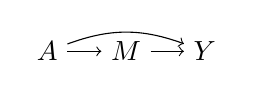
\begin{tikzpicture}
    % x node set with absolute coordinates
    \node (a) at (0,0) {$A$};
    \node (m) at (1,0) {$M$};
    \node (y) at (2,0) {$Y$};
    \path[->] (a) edge (m);
    \path[->] (m) edge (y);
    \path[->, bend left=20] (a) edge (y);
\end{tikzpicture}} seen as longitudinal with  $k_0$: $A$ and $k_1$: $M$


\textbf{decompose} $\mathrm{E}\left[Y^{a=1}\right]  - \mathrm{E}\left[Y^{a=0}\right]$ into cross-world quantities
\begin{itemize}[itemsep=0em, topsep=0pt, partopsep=0pt,parsep=0pt, leftmargin=1.5em]
\item pure (aka natural) direct effect (upper path) $$\mathrm{E}\left[Y^{a=1, M^{a=0}}\right]  - \mathrm{E}\left[Y^{a=0, M^{a=0}}\right]$$
\item total (aka natural) indirect effect (lower path) $$\mathrm{E}\left[Y^{a=1, M^{a=1}}\right]  - \mathrm{E}\left[Y^{a=1, M^{a=0}}\right]$$
\end{itemize}

\textbf{mediation formula} under NPSEM-IE (requires $Y^{a=1,m} \indep M^{a=0}$ cross-world independence)
$$\mathrm{E}\left[Y^{a=1,M^{a=0}}\right] = \sum_m \mathrm{E}\left[Y|A=1, M=m\right]\mathrm{Pr}\left[M=m|A=0\right] $$


\textbf{interventional interpretation} advocating NPSEM-IE assuming:
\trimbox{0cm 0.095cm 0cm 0cm}{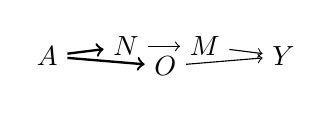
\begin{tikzpicture}
    % x node set with absolute coordinates
    \node (a) at (-1,0.125) {$A$};
    \node (n) at (0,0.25) {$N$};
    \node (o) at (0.5,0) {$O$};
    \node (m) at (1,0.25) {$M$};
    \node (y) at (2,0.125) {$Y$};
    \path[->, line width=0.3mm] (a) edge (n);
    \path[->] (n) edge (m);
    \path[->] (m) edge (y);
    \path[->, line width=0.3mm] (a) edge (o);
    \path[->] (o) edge (y);
\end{tikzpicture}}
(thick arrows are deterministic)

no controlled direct effects: no $N\to Y$ and no $O\to M$

FFRCISTG point of view: intervention on $N$ and $O$ separately

if decomposable (can be verified in a randomized trial), g-formula for $N$ and $O$ reduces to mediation formula for $A$



\end{minipage}}

\end{multicols}


%-------------------------------------------------------------------------------

% SECTION: MODELS

%-------------------------------------------------------------------------------

\section{Models}

\begin{multicols}{2}

\paragraph{Modeling} data are a sample from the target population \vspace{0.4em}

\noindent \hspace{0.9em}\begin{tabular}{l l l}
\textbf{\it estimand:} & quantity  of interest, & e.\,g.\ $\mathrm{E}\left[Y|A=a\right]$ \\
\textbf{\it estimator:} & function to use, & e.\,g.\ $\widehat{\mathrm{E}}\left[Y|A=a\right]$ \\
\textbf{\it estimate:} & apply function to data, & e.\,g.\ $4.1$ 
\end{tabular} \vspace{0.5em}

\noindent \textbf{model}: a priori restriction of joint distribution/dose-response curve;  \textit{assumption:} no model misspecification (usually wrong)

\noindent \textbf{non-parametric estimator:} no restriction (saturated model) $=$ \textit{Fisher consistent estimator} (entire population data $\rightarrow$ true value)

\noindent \textbf{parsimonious model:} few parameters estimate many quantities

\noindent \textbf{bias-variance trade-off:} \newline wiggliness $\uparrow$ $\rightarrow$ misspecification bias $\downarrow$, CI width $\uparrow$

\paragraph{Variable Selection} can induce bias if $L$ includes: 

\hspace{-0.2em}\vspace{-1em}
\begin{tabular}{l l }
 (decendant of) collider:& \textit{selection bias under the null}\\
 noncollider effect of $A$:& \textit{selection bias under the alternative}\\
 mediator:& \textit{overadjustment for mediators}
\end{tabular}

\noindent temporal ordering is not enough to conclude anything

\noindent \textbf{bias amplification:} e.\,g.\ by adjusting for an instrument $Z$ (can also reduce bias)



\paragraph{Super Learning} \citep{van2007super, van2011targeted}

\noindent \textbf{oracle selector:} select best estimator of set of learners $Z_i$

\noindent \textbf{discrete super learner:} select algorithm with smallest cross-validated error (converges to oracle for large sample size)

\noindent \textbf{super learner:} improves asymptotically on discrete version

$\mathrm{logit} (Y=1|Z) = \sum_i \alpha_i Z_i, $ with $0<\alpha_i<1$ and $\sum\alpha_i=1$
weights $\alpha_i$ are determined inside the cross-validation; for the prediction, $Z_i$ trained on the full data set are used

\noindent   can be cross-validated itself to check for overfitting (unlikely)


\paragraph{Marginal Structural Models} association is causation in the IP weighted pseudo-population 
$$\text{associational model } \mathrm{E}\left[Y|A\right] = \text{ causal model } \mathrm{E}\left[Y^a\right]$$

\noindent \textit{step 1:} estimate/model $f\left[A|L\right]$ (and $f\left[A\right]$) $\rightarrow$ get $(S)W^A$

\noindent \textit{step 2:} estimate regression parameters for pseudo-population

\noindent \textbf{effect modification} variables $V$ can be included (e.\,g.\ $\beta_0+\beta_1 a+\beta_2 V a + \beta_3 V$; technically not marginal anymore), $SW^A(V) = \frac{f\left[A|V\right]}{f\left[A|L\right]}$ more efficient than $SW^A$
 










\end{multicols}

\subsection{Traditional Methods}

\begin{multicols}{2}




\paragraph{Stratification}  calculate risk for each stratum of $L$

\noindent only feasible if enough data per stratum


\paragraph{Outcome Regression} often assume no effect modification
$$\mathrm{E}\left[Y^{a,c=0}|L\right] = \beta_0 + \beta_1 a + \beta_2 aL +\beta_3 L = \mathrm{E}\left[Y|A, C=0, L\right]$$

\noindent faux marginal structural model as no IP weighting/$SW^A(L)=1$

\noindent for ATE only $\beta_1,\beta_2$ of interest, the rest are \textit{nuisance parameters}

\paragraph{Propensity Score Methods}
$\mathrm{Pr}\left[A=1|L\right] =: \pi(L)$ 
 
\noindent  $\Rightarrow A\indep L|\pi(L)$ (definition of a  balancing score); can be modelled  


\begin{itemize}[itemsep=0em, topsep=0pt, partopsep=0pt,parsep=0pt, leftmargin=1.5em]
\setlength{\itemsep}{0pt}%
\setlength{\parskip}{0pt}
\item \textit{\textbf{stratification:}} create strata with similar $\pi(L)$ (e.\,g.\ deciles), but the average $\pi(L)$ might still be different in some strata
\item \textit{\textbf{standardization:}} use $\pi(L)$ instead of $L$ to standardize
\item \textit{\textbf{matching:}} find close ($\rightarrow$ bias-variance trade-off) values of $\pi(L)$, positivity issues arise often
\end{itemize}

\noindent propensity models don't need to predict well, just ensure exchangeability (good prediction leads to positivity problems)


\paragraph{Instrumental Variable Estimation} $L$ unmeasured

\noindent surrogate/proxy instruments can be used

\noindent \textbf{instrumental conditions:} 
\begin{enumerate}[itemsep=0em, topsep=0pt, partopsep=0pt,parsep=0pt, leftmargin=1.5em]
\setlength{\itemsep}{0pt}%
\setlength{\parskip}{0pt}
\item \textbf{\textit{relevance condition:}} $Z \not\!\indep A$, meaning $Z$ is associated with $A$ \newline (weak association (F-statistic $< 10$) $\rightarrow$ weak instrument)
\item \textbf{\textit{exclusion restriction:}} $Z$ affects $Y$ at most through $A$
\begin{enumerate}[itemsep=0em, topsep=0pt, partopsep=0pt,parsep=0pt, leftmargin=1.5em]
\setlength{\itemsep}{0pt}%
\setlength{\parskip}{0pt}
\item population level: $\mathrm{E}\left[Y^{z,a}\right] = \mathrm{E}\left[Y^{z',a}\right]$ (sometimes enough)
\item \textbf{\textit{individual level:}} $Y^{z,a}_i =  Y^{z',a}_i = Y^{a}_i$
\end{enumerate}
\item \textbf{\textit{exchangeability:}} $Z$ and $Y$ have no shared causes
\begin{enumerate}[itemsep=0em, topsep=0pt, partopsep=0pt,parsep=0pt, leftmargin=1.5em]
\setlength{\itemsep}{0pt}%
\setlength{\parskip}{0pt}
\item \textbf{\textit{marginal:}} $Y^{a,z} \indep Z$ (typically enough)
\item joint: $\left\{Y^{z, a};a\in\left[0,1\right],z\in\left[0,1\right]\right\} \indep Z$
\end{enumerate}
\item  (not needed for an instrument, just the IV estimand below)
\begin{enumerate}[itemsep=0em, topsep=0pt, partopsep=0pt,parsep=0pt, leftmargin=1.5em]
\setlength{\itemsep}{0pt}%
\setlength{\parskip}{0pt}
\item \textit{effect homogeneity:} (i) constant effect $A\rightarrow Y \,\, \forall i$ (ii) constant average effect $A\rightarrow Y \,\, \forall A$ (iii) no additive effect modifiers (iv) additive Z-A association is constant across $L$
\item \textit{monotonicity:} $A^{z=1} \geq A^{z=0} \,\, \forall i$ (more credible than 4a)
\end{enumerate}
\end{enumerate}

\noindent \textbf{common instruments:} (physician's) general preference, access to/price of $A$, genetic factors (Mendelian randomization)

\noindent \textbf{bounds:} binary outcome ATE $\left[-1,1\right]$ (width 2)  $\overset{data}{\rightarrow}$ (width 1)

\noindent \textit{natural bounds} need 2a,3a  (width $\mathrm{Pr}\left[A{=}1|Z{=}0\right] + \mathrm{Pr}\left[A{=}0|Z{=}1\right]$)

\noindent \textit{sharp bounds} require 2a,3b (narrower than natural bounds)


\noindent \textbf{IV estimand ATE}: intention-to-treat $\div$ measure of compliance

\noindent (1,2b,3a,4a):  ATE;
  (1,2b,3a,4b): ATE in compliers

\noindent binary $Z$: $\frac{\mathrm{E}\left[Y|Z=1\right] - \mathrm{E}\left[Y|Z=0\right]}{\mathrm{E}\left[A|Z=1\right] - \mathrm{E}\left[A|Z=0\right]}$, continuous $Z$: $\frac{Cov(Y,Z)}{Cov(A,Z)}$; \newline can be calculated as \textit{two-stage-least-squares estimator:} \newline 1.\ $\mathrm{E}\left[A|Z\right]$ 2.\ $\mathrm{E}\left[Y|Z\right] = \beta_0 + \beta_1\hat{\mathrm{E}}\left[A|Z\right]$ 3. $\hat{\beta}_1$ is IV estimate

\noindent \textbf{disadvantages:} often leads to wide CI, small violations of conditions can lead to large biases

\noindent \textbf{regression discontinuity design:} if threshold in $L$ exists which determines $A$ perfectly + assumption of continuity in $L$ $\to$ jump in $Y$ at threshold is the causal effect (if no effect modification by $L$); a fuzzy variant also exists
\citep{hernan2023causal}



\paragraph{Causal Survival Analysis} time-to-event data

\noindent additional censoring due to administrative end of follow-up

\noindent \textbf{competing events} (often death): censoring (assume population with death abolished) or not (after death, chance of event is zero, but what is the effect of $A$?) $\rightarrow$ create composite event

\noindent \textbf{survival quantities} $k$ is a time point, $T$ is time of event
\begin{itemize}[itemsep=0em, topsep=0pt, partopsep=0pt,parsep=0pt, leftmargin=1.5em]
\setlength{\itemsep}{0pt}%
\setlength{\parskip}{0pt}
\item \textit{survival} at $k$: $\mathrm{Pr}\left[T>k\right] =:\mathrm{Pr}\left[D_k=0\right]$
\item \textit{risk} at $k$: $1-\mathrm{Pr}\left[T>k\right] = \mathrm{Pr}\left[T \leq k\right] = \mathrm{Pr}\left[D_k=1\right]$
\item \textit{hazard} at $k$: $\mathrm{Pr}\left[T=k|T> k{-}1\right] =\mathrm{Pr}\left[D_k=1|D_{k{-}1}=0\right]$, \textit{hazard ratio} is paradoxical due to  in-built selection bias
\end{itemize}

\noindent \textbf{modeling:} some options
\begin{itemize}[itemsep=0em, topsep=0pt, partopsep=0pt,parsep=0pt, leftmargin=1.5em]
\setlength{\itemsep}{0pt}%
\setlength{\parskip}{0pt}
\item \textit{\textbf{Kaplan-Meier}} aka product limit formula (nonparametric): $\mathrm{Pr}\left[D_k=0\right] = \prod_{m=1}^k \mathrm{Pr}\left[D_m=0|D_{m-1}=0\right]$
\item parametric e.\,g.\ log hazards model: 
\begin{itemize}[itemsep=0em, topsep=0pt, partopsep=0pt,parsep=0pt, leftmargin=1.5em]
\setlength{\itemsep}{0pt}%
\setlength{\parskip}{0pt}
\item use \textit{\textbf{IP weigths}} $SW^A$ in structural marginal model $\mathrm{logit} \: \mathrm{Pr}\left[D_{k+1}^{a, \bar{c}=\bar{0}}=0|D_{k}^{a, \bar{c}=\bar{0}}=0\right] = \beta_{0,k} + \beta_1a+\beta_2ak $
\item \textit{\textbf{standardize}} ($\prod_k 1-$) parametric hazards model $\mathrm{Pr}\left[D_{k+1}=1|D_k = 0, C_k=0, L, A\right]$ weighting across $L$
\end{itemize}
\item \textit{\textbf{structural nested cumulative failure time model (CFT):}}
$\frac{\mathrm{Pr}\left[D_k^a=1|L,A\right]}{\mathrm{Pr}\left[D_k^{a=0}=1|L,A\right]} = \exp\left[\gamma_k(L,A;\psi)\right]$ (log-linear has no upper limit 1 $\rightarrow$ rare failure $\uparrow$; if $\downarrow$, use a survival model (CST)), use g-estimation like with AFT
\item \textit{\textbf{accelerated failure time model (AFT)}} with g-estimation: $T_i^a/T_i^{a=0} = \exp(-\psi_1a -\psi_2aL_i)$, exchangeability for $C$ is guaranteed via artificial censoring (include only individuals who would not have been censored either way) 
\end{itemize}



\vspace{0.2em}
\noindent \colorbox{lightgray!20!white}{\begin{minipage}{28em}




\textbf{\textcolor{darkgray}{time-varying}} two options based on g-methods as examples

\noindent \textbf{standardization} (plug-in estimate): risk is $\mathrm{Pr}\left[D_{k+1}^{\bar{a},\bar{c}=\bar{0}}=1\right] =$ \vspace{-0.5em}
\begin{align*}%{3}
 \sum_{\bar{l}_k}&\sum_{j=0}^k \mathrm{Pr}\left[D_{j+1}=0|\bar{A}_j=\bar{a}_j, \bar{L}_j=\bar{l}_j, \bar{D}_j=0\right] \times \\[-0.1em]
\prod_{s=0}^j & \Big\{  \mathrm{Pr}\left[D_s=0|\bar{A}_{s-1}=\bar{a}_{s-1}, \bar{L}_{s-1}=\bar{l}_{s-1}, \bar{D}_{s-1}=0\right] \times  \\[-0.7em]
   &   \,\,\,\,\, f\left(l_s|\bar{a}_{s-1}, \bar{l}_{s-1}, D_s=0\right)\Big\}
\end{align*}
\noindent \textbf{IP weighting:} fit a pooled logistic hazard model with time-varying weights
$W^{\bar{A}}_k =\prod_{m=0}^k\frac{1}{f(A_m|\bar{A}_{m-1}, \bar{L}_m)}$



\end{minipage}}



\end{multicols}


%-------------------------------------------------------------------------------

% SECTION: G-METHODS

%-------------------------------------------------------------------------------

\subsection{G-Methods}
\begin{multicols}{2}


\paragraph{G-Methods} \textit{g}eneralized treatment contrasts:
adjust for $L$
\begin{itemize}[itemsep=0em, topsep=0pt, partopsep=0pt,parsep=0pt]
\setlength{\itemsep}{0pt}%
\setlength{\parskip}{0pt}
\item \textbf{\textit{standardization:}}  two types of g-formula
\item \textbf{\textit{IP weighting:}} (in theory) also g-formula 
\item \textbf{\textit{g-estimation:}} not needed unless longitudinal
\end{itemize}

\noindent \textbf{standardization and IP weighting}
are equivalent, \textit{\textbf{but}} if modeled, different ``no misspecification'' assumptions: outcome model (standardization), treatment model (IP weighting)

\noindent \textbf{big g-formula}
not all methods use (sequential) exchangeability 
\begin{itemize}[itemsep=0em, topsep=0pt, partopsep=0pt,parsep=0pt]
\item \textit{problem:} DAG is known, but unmeasured variables exist
\item \textit{solution:} include un- \& measured variables in big g-formula $\to$ derive
alternative effect identification methods using only d-separation (e.\,g.\  front door formula)
\end{itemize}
it can always be determined, if the DAG allows for identification with the big g-formula
\citep{hernan2023causal}


\noindent \textbf{censoring:} measure joint effect of $A$ and $C$ with
$\mathrm{E}\left[Y^{a, c=0}\right]$

\noindent \textit{standardization} $\mathrm{E}\left[Y|A=a\right] = \int \mathrm{E}\left[Y|L{=}l, A{=}a, C{=}0\right]dF_L\left[l\right]$\vspace{0.2em}

\noindent \textit{IP weights}\vspace{-1.30em}

\hspace{3.5em}\begin{tabular}{l l l}
$W^{A,C}=W^A \times W^C$  &(uses $n$) & or \\
$SW^{A,C}=SW^A \times SW^C$ &(uses $n^{c=0}$) & 
\end{tabular}\vspace{0.3em}

\noindent \textit{g-estimation} only adjusts for confounding  $\rightarrow$ use IP weights

\vspace{0.2em}
\noindent \colorbox{lightgray!20!white}{\begin{minipage}{28em}

\textbf{\textcolor{darkgray}{time-varying}} censoring $\bar{C}$: monotonic type of missing data 

\noindent \textbf{standardization}: $\!\!\!\displaystyle\int\!\! f(y|\bar{a}, \bar{c}{=}\bar{0}, \bar{l}) \prod\limits_{k=0}^K dF\left(l_k|\bar{a}_{k-1}, c_{k-1} {=} 0, \bar{l}_{k-1}\right)$

\noindent \textbf{IP weighting}:
\noindent $$\textcolor{gray}{S}W^{\bar{C}}= \prod_{k=1}^{K+1}\frac{1\textcolor{gray}{\cdot \mathrm{Pr}\left(C_k=0|\bar{A}_{k-1}, C_{k-1}=0\right)}}{\mathrm{Pr}\left(C_k=0|\bar{A}_{k-1}, C_{k-1}=0, \bar{L}_k\right)} $$

\end{minipage}}




\paragraph{Standardization} plug-in (parametric if so) g-formula
$$\mathrm{E}\left[Y^{a}\right] = \overbrace{\mathrm{E}\left[\mathrm{E}\left[Y|A{=}a,L{=}l\right]\right]}^{\text{conditional expectation}} =  \overbrace{ \textstyle{\int} \mathrm{E}\left[Y|L=l, A=a\right]f_L\left[l\right]dl}^{\text{joint density estimator}} $$
weighted average of stratum-specific risks; unknowns can be estimated non-parametrically or modeled

\noindent \textbf{no need to estimate $\boldsymbol{f_L\left[l\right]}$/integrate} as empirical distribution can be used: estimate outcome model $\rightarrow$ predict counterfactuals on whole dataset $\rightarrow$ average the results ($\rightarrow$ CI by bootstrapping)

\noindent \textbf{for discrete $\boldsymbol{ L}$}  $\mathrm{E}\left[Y|A=a\right] = \sum_l \mathrm{E}\left[Y|L=l, A=a\right]\mathrm{Pr}\left[L=l\right]$

\vspace{0.2em}
\noindent \colorbox{lightgray!20!white}{\begin{minipage}{28em}

\textbf{\textcolor{darkgray}{time-varying}} standardize over all possible $\bar{l}$-histories



\noindent simulates joint distribution of counterfactuals $\left(Y^{\bar{a}}, \bar{L}^{\bar{a}}\right)$ for $\bar{a}$
\textbf{joint density estimator (jde)}
\begin{align*}
& \text{discrete: } \mathrm{E}\left[Y^{\bar{a}}\right] = \sum_{\bar{l}} \mathrm{E}\left[Y|\bar{A}=\bar{a}, \bar{L}=\bar{l} \right] \prod_{k=0}^K f \left(l_k|\bar{a}_{k-1}, \bar{l}_{k-1}\right)  \\ &
\text{continuous: } \int f(y|\bar{a}, \bar{l}) \prod_{k=0}^K f\left(l_k|\bar{a}_{k-1}, \bar{l}_{k-1}\right)dl
\end{align*}

\noindent for \textit{stochastic strategies} multiply with $\prod_{k=0}^K f^{int} \left(a_k|\bar{a}_{k-1}, \bar{l}_{k}\right) $

\end{minipage}}

\noindent \colorbox{lightgray!20!white}{
\begin{minipage}{28em}


\begin{mdframed}[linecolor=black!20!,
    outerlinewidth=0.2pt,
    innertopmargin=0.5\baselineskip,
    innerbottommargin=0.5\baselineskip,
    backgroundcolor=lightgray!20!white, innerleftmargin=2pt, innerrightmargin=2pt]
\textbf{estimation} \citep{young2011comparative, schomaker_using_2019}

\begin{enumerate}[itemsep=0em, topsep=0pt, partopsep=0pt,parsep=0pt, leftmargin=1.5em]
\setlength{\itemsep}{0pt}%
\setlength{\parskip}{0pt}
\item model $f \left(l_k|\bar{a}_{k-1}, \bar{l}_{k-1}\right)$ and $\mathrm{E}\left[Y|\bar{A}=\bar{a}, \bar{L}=\bar{l} \right]$
\item simulate data forward in time: \newline
at $k=0$: use empirical distribution of $L_0$ (observed data) \newline
at $k>0$: set $\bar{A} = \bar{a}$, \textit{draw} from models estimated in 1.
\item calculate mean of $\hat{Y}_{K,i}^{\bar{a}}$ (bootstrap for CI)
\end{enumerate}

\end{mdframed}





\textbf{iterated conditional expectation (ice)} 
$$\mathrm{E}\left[ Y_T^{\bar{a}}\right] = \mathrm{E} \left[ \mathrm{E} \left[\mathrm{E} \left[ ... \mathrm{E} \left[Y_T| \bar{A}_{T{-}1} {=} \bar{a}_{T{-}1}, \bar{L}_T \right]  ...|\bar{A}_0 {=} a_0, L_1 \right] |L_0 \right]\right]$$



\begin{mdframed}[linecolor=black!20!,
    outerlinewidth=0.2pt,
    innertopmargin=0.5\baselineskip,
    innerbottommargin=0.5\baselineskip,
    backgroundcolor=lightgray!20!white, innerleftmargin=2pt, innerrightmargin=2pt]
\textbf{estimation} \citep{schomaker_using_2019}

\begin{enumerate}[itemsep=0em, topsep=0pt, partopsep=0pt,parsep=0pt, leftmargin=1.5em]
\setlength{\itemsep}{0pt}%
\setlength{\parskip}{0pt}
\item model inside out: $Q_{T} {=} \mathrm{E} \left[Y_T| \bar{A}_{T{-}1}, \bar{L}_T \right]$ to $Q_0 {=} \mathrm{E} \left[Q_1| \bar{L}_0 \right]$, predict $Q_t$ with $\bar{A} = \bar{a}$ in each step
\item calculate mean of $\hat{Q}_{0,i}^{\bar{a}}$ (bootstrap for CI)
\end{enumerate}



\end{mdframed}

\noindent \textbf{g-null paradox} even if the sharp null holds, model misspecification can lead to it being falsely rejected

\end{minipage}}



\begin{mdframed}[style=MyFrame,nobreak=true, innerleftmargin=2pt, innerrightmargin=2pt]
Proof: for $L_0 \rightarrow A_0 \rightarrow Y_0 \rightarrow L_1 \rightarrow A_1 \rightarrow Y_1$, $\bar{a} =(a_0,a_1)$ 
\begin{alignat*}{4} 
\mathrm{E}\left[Y_1^{\bar{a}}\right] & \overset{\text{CE}}{=} && \mathrm{E}\left[\mathrm{E}\left[   Y_1^{\bar{a}}|A_0{=}a_0, L_0   \right]\right]  \\ 
\text{(ice)}\,\,\, &\overset{\text{CE*}}{=} && \mathrm{E}\left[\mathrm{E}\left[  \mathrm{E}\left[Y_1|\bar{L}, \bar{A}{=}\bar{a}, Y_0 \right]| A_0{=}a_0, L_0   \right]\right]  \\ 
&\overset{\text{LTP}}{=} && \mathrm{E}\left[ \sum\nolimits_{l_1} \mathrm{E}\left[Y_1|A_0{=}a_0, \bar{L}, Y_0\right] \mathrm{Pr}\left[l_1|a_0,l_0, y_0\right]         \right] \\
&\overset{\text{LTP}}{=} && \sum\nolimits_{l_0}\!\!\!\left[ \sum\nolimits_{l_1} \!\!\!\mathrm{E}\left[Y_1|A_0{=}a_0, \bar{L}, Y_0\right] \mathrm{Pr}\left[l_1|a_0,l_0, y_0\right]         \right] \mathrm{Pr}\left[l_0\right] \\
\text{(jde)}\,\,\, &\overset{\text{sum}}{=} &&  \sum\nolimits_{\bar{l}} \mathrm{E}\left[Y_1|A_0{=}a_0, \bar{L}, Y_0\right] \mathrm{Pr}\left[l_1|a_0,l_0\right]          \mathrm{Pr}\left[l_0\right] 
\end{alignat*}
CE: conditional expectation; *: exchangeability; \newline LTP: law of total probability
\end{mdframed}







\paragraph{IP Weighting} \textit{i}nverse \textit{p}robability of treatment (g-formula)
$$\mathrm{E}\left[Y^{a}\right] = \mathrm{E}\left[\frac{I(A=a)Y}{f\left[A|L\right]}\right]; W^A=\frac{1}{f\left[A|L\right]}; SW^A = \frac{f(A)}{f\left[A|L\right]}$$

\noindent unknowns can be estimated non-parametrically or modeled
\noindent \textbf{pseudo-population:} everyone is treated \& untreated ($L\not\to A$)

\noindent \textbf{FRCISTG} \textit{(fully randomized causally interpreted structured graph)}: probability tree for $L \rightarrow A \rightarrow Y$, can be used to calculate/visualize simulation of values for $A$ 

\noindent \textbf{for discrete $\boldsymbol{A, L}$:} $f\left[a|l\right] = \mathrm{Pr}\left[A=a,L=l\right]$

\noindent \textbf{estimators:} Horvitz-Thompson; Hajek (modified version) %todo p.152 

\noindent \textbf{stabilized weights $\boldsymbol{SW^A}$} should have an average of 1 (check!) $\rightarrow$ pseudo-population same size $\rightarrow$ CI width $\downarrow$

\vspace{0.2em}
\noindent \colorbox{lightgray!20!white}{\begin{minipage}{28em}




\textbf{\textcolor{darkgray}{time-varying}}
$$ W^{\bar{A}} = \prod_{k=0}^K \frac{1}{f\left(A_k|\bar{A}_{k-1}, \bar{L}_k\right)}; \,\,\,\, SW^{\bar{A}} = \prod_{k=0}^K \frac{f\left(A_k|\bar{A}_{k-1}\right)}{f\left(A_k|\bar{A}_{k-1}, \bar{L}_k\right)}$$

\end{minipage}}



















\paragraph{G-Estimation} (additive) structural nested models %todo: verbesserung von allem, ich habs noch nicht ganz verstanden
\begin{align*}
\mathrm{logit} \, \mathrm{Pr}\left[A=1|H(\psi^\dagger), L\right] &= \alpha_0 + \alpha_1H(\psi^\dagger) + \alpha_2L \\
H(\psi^\dagger) &= Y - \psi_\dagger A
\end{align*}
find $\psi^\dagger$ which renders $\alpha_1=0$; 95\,\%-CI: all $\psi^\dagger$ for which $p>0.05$
closed-form solution for linear models


\noindent \textbf{derivation:} $H(\psi^\dagger) = Y^{a=0}$
$$\mathrm{logit} \, \mathrm{Pr}\left[A=1|Y^{a=0}, L\right] = \alpha_0 + \alpha_1Y^{a=0} + \alpha_2L$$
$Y^{a=0}$ unknown, but because of exchangeability $\alpha_1$ should be zero
$$Y^{a=0} =Y^a - \psi_1 a$$
equivalent to $Y^{a=0} =Y^{a=1} - \psi_1$, but using no counterfactuals



\noindent \textbf{structural nested mean model}
\begin{align*}
\text{additive: }\,\,\, & \mathrm{E}\left[Y^a-Y^{a=0}|A=a, L\right] &= \beta_1 a \,(+ \beta_2 a L) \\
\text{multiplicative: }\,\,\, & \log \left( \frac{\mathrm{E}\left[Y^a|A=a, L\right]}{\mathrm{E}\left[Y^{a=0}|A=a, L\right]} \right) &= \beta_1 a \,(+ \beta_2 a L)
\end{align*} 
multiplicative is preferred if $Y$ always positive, but does not extend to longitudinal case

\noindent semi-parametric: agnostic about $\beta_0$ and effect of $L$ $\rightarrow$ robust $\uparrow$

\noindent \textbf{no time-varying:} no nesting; model equals marginal structural models with missing $\beta_0, \beta_3$ (unspecified ``no treatment'')

\noindent \textbf{sensitivity analysis:} unmeasured confounding ($\alpha_1 \neq 0$) can be examined: do procedure  for different values of $\alpha_1$ $\rightarrow$ plot $\alpha_1$ vs.\ $\psi^\dagger$ $\rightarrow$ how sensitive is  estimate to unmeasured confounding?

\noindent \textbf{effect modification:} add $V$ in both g-estimation equations %todo


\noindent \textbf{doubly robust estimators} exist%todo

\vspace{0.2em}
\noindent \colorbox{lightgray!20!white}{\begin{minipage}{28em}
\textbf{\textcolor{darkgray}{time-varying}}
 nested equations: for each time $k$

\noindent \textbf{strutural nested mean models} separate effect of each $a_k$
$$\mathrm{E}\left[Y^{\bar{a}_{k-1}, a_k, \underline{0}_{k+1}} - Y^{\bar{a}_{k-1}, \underline{0}_{k+1}}|\bar{L}^{\bar{a}_{k-1}}=\bar{l}_k, \bar{A}_{k-1} = \bar{a}_{k-1}\right] = $$
$$  a_k\gamma_k\left(\bar{a}_{k-1}, \bar{l}_k,\beta\right)$$
\noindent \textbf{calculations}
$$H_k\left(\psi^\dagger\right) = Y - \sum_{j=k}^K A_j \gamma_j\left(\bar{A}_{j-1}, \bar{L}_j, \psi^\dagger\right)$$
\noindent function $\gamma_j$ can be, e.\,g.\ constant ($\psi_1$), time-varying only ($\psi_1+\psi_2k$), or dependent on treatment/covariate history
$$\mathrm{logit}\,\mathrm{Pr}\left[A_k=1|H_k\left(\psi^\dagger\right), \bar{L}_k,\bar{A}_{k-1}\right]=$$
$$\alpha_0 +\alpha_1H_k\left(\psi^\dagger\right)+\alpha_2 w_k\left(\bar{L}_k,\bar{A}_{k-1}\right)
$$
find $\alpha_1$ that is closest to zero

a closed form estimator exists for the linear case

\end{minipage}}

























\end{multicols}



\subsection{Doubly Robust Methods}

\begin{multicols}{2}



%todo p 280-283, 284


\paragraph{Double-Robustness} \citep{hernan2023causal}

\noindent g-formula: \textit{either} treatment model $f(L)$  \textit{or} outcome model $b(L)$ 

\noindent \textit{\textbf{or}} appropriately combine both: ``two chances to get it right''

\noindent \textbf{all doubly robust estimators} 
\begin{itemize}[leftmargin=*, itemsep=0em, topsep=0pt, partopsep=0pt,parsep=0pt]
\item involve a correction of  outcome $\hat{b}(L)$ using the treatment $\hat{f}(L)$
\item have a bias depending on a product of the errors $\frac{1}{\pi(l)} - \frac{1}{\hat{\pi}(l)}$ and $b(l) - \hat{b}(l)$ known as second order bias 
%(as discussed in chapter 18, this allows machine learning, as machine learning will get that bias smaller than other things in high-dimensional cases)
\end{itemize}

\vspace{0.2em}
\noindent \colorbox{lightgray!20!white}{\begin{minipage}{28em}

\textbf{\textcolor{darkgray}{time-varying:}} 
  multiple robustness for $k=0,1,...K$
  
 $K{+}\,2$ robustness: consistent, if $\hat{f}_0$ to $\hat{f}_l$ and $\hat{b}_{l+1}$ to $\hat{b}_K$ are 
 
 $2^{K{+}1}$ robustness: consistent, if for each k, either  $\hat{f}_k$ or $\hat{b}_k$ are
  
  \end{minipage}}

\paragraph{Machine Learning} $L$ is high-dimensional

\noindent one could use lasso or ML for IP weighting/standardization

\noindent \textbf{\textit{but:}} ML does not guarantee elimination of confounding and has largely unknown statistical properties: how to get CI?

\noindent \textbf{sample splitting:} train estimators on training sample $T_r$, use resulting estimators for doubly robust method on estimation sample (CIs on estimation sample are valid, but $n$ halved)

\noindent \textbf{cross-fitting:} do again the other way round, average the two estimates, get CI via bootstrapping
[\textit{alternatively:} split into $M$ samples, use one sample for estimation and $M{-}1$ for training $\to$ improved finite sample behavior \citep{hernan2023causal}]



%todo p.240 - 244
\noindent \textbf{asymptotic behavior} 
for valid (Wald) CI we need:
\begin{itemize}[leftmargin=*, itemsep=0em, topsep=0pt, partopsep=0pt,parsep=0pt]
\item a bias  much smaller than $c \cdot 1/\sqrt{n}$, which is how the $se$ typically scales (use doubly robust methods for small bias)
%Wald CI for $\mathrm{E}\left[Y^a\right] $ standard error typically scales as $c \cdot 1/\sqrt{n}$, therefore, the bias needs to be much less for valid CI 
\item asymptotic normality (for Wald CI)
\item for a doubly robust estimator $\psi_{dr}$, we need sample splitting, otherwise $\hat{b}(l)$ and $\hat{f}(l)$ are correlated with $\psi_{dr}$
\end{itemize}

\noindent if $\hat{b}(l)$ and $\hat{f}(l)$ are consistent and $\mathrm{E}[\hat{\psi} - \psi|T_r]/se(\hat{\psi})$ converges to 0 $\to$ $\hat{\psi}$ with sample splitting is asymptotically normal and unbiased $\to$ CI is calibrated
\citep{hernan2023causal}


\noindent \textbf{problems:} unclear choice of algorithm, is bias small enough?

\paragraph{Advantages} \citep{van2011targeted}

\noindent \textbf{consistent} \textit{if either $\bar{Q}_0$ or $g_n$ are consistent (doubly robust)}:
$$\forall \epsilon>0, P \in \mathcal{M}: \mathrm{Pr}_P\left[|\hat{\theta}_n-\theta(P)|>\epsilon\right] \to 0 \text{ as } n\to\infty$$

\noindent \textbf{collaboratively doubly robust:} $g_n$ only needs predictors of $Y$, as it does not try to fit $g_0$ well, but improve the fit of $\bar{Q}^*_n$

\noindent \textbf{asymptotic unbiasedness}
\textit{if either $\bar{Q}_0$ or $g_0$ are consistent}, super learning makes $\bar{Q}_0$ and $g_n$ max.\ asymptotically unbiased

\noindent \textbf{asymptotic efficiency} \textit{if both $\bar{Q}_0$ and $g_n$ are consistent}: achieves Cramer-Rao bound of minimum possible asymptotic variance (requires asymptotic unbiasedness)

\noindent \textbf{asymptotic linearity} \textit{if either  $\bar{Q}_0$ or $g_n$ are consistent}: \newline means estimator behaves like empirical mean
\begin{itemize}[leftmargin=*, itemsep=0em, topsep=0pt, partopsep=0pt,parsep=0pt]
\setlength{\itemsep}{0pt}%
\setlength{\parskip}{0pt}
\item bias converges to zero at rate smaller than $1/\sqrt{n}$
\item for large $n$ estimator is approximately normally distributed
\end{itemize}

\paragraph{Influence Curve} how robust is an estimator? %\citep{hampel1974influence, van2011targeted}
$$IC_{T,P_n}(O)=\lim_{\epsilon\to 0}\frac{T\left[\left(1-\epsilon\right)P_n + \epsilon\delta_O\right]-T(P_n)}{\epsilon}$$
for estimator $T$ and distribution $P_n$ with $0<\epsilon<1$ 


\noindent can also be rewritten as a \textit{\textbf{directional derivative}} at $P_n$
$$IC_{T,P_n}=\frac{d}{d\epsilon}T\left[\left(1-\epsilon\right)P_n + \epsilon\delta_O\right] = 
\frac{d}{dP_n}T\left(\delta_O - P_n\right)$$
in direction $(\delta_O - P_n)$, where $P_n$ empirical probability measure that puts mass $1/n$ on $O_i$ \citep{hampel1974influence}


\noindent \textbf{special cases} \citep{van2011targeted}
\begin{itemize}[leftmargin=*, itemsep=0em, topsep=0pt, partopsep=0pt,parsep=0pt]
\item $\overline{IC}(P_0) = 0$ and $\mathrm{Var}(IC(P_0))$ asymptotic variance of the standard estimator  $\sqrt{n} (\psi_n - \psi_0)$, $\to$ $Var(\hat{\Psi}(P_n)) = \frac{Var_{IC}}{n}$
\item efficient IC: an estimator is asymptotically efficient $\Leftrightarrow$ its influence curve is the efficient influence curve $IC(O)=D^*(O)$ 
\end{itemize}





\paragraph{Delta Method}  \citep{zepeda2022delta} estimand is a function of $\theta$, i.e. $\psi := \phi(\theta)$, $Var(\hat{\theta})$ known, but what is $Var(\hat{\psi})$?


\noindent \textbf{Taylor's approximation} requirements:
\begin{itemize}[leftmargin=*, itemsep=0em, topsep=0pt, partopsep=0pt,parsep=0pt]
\item univariate $\phi$: differentiable at $\theta$
\item multivariate $\phi$: $\exists$ $\partial_v\phi(\theta)$ (directional derivative)
\item functional $\phi$ (function of functions): $\exists$ $\partial_v\phi(\theta)$ \& coincides with one-sided directional (Hadamard) derivatives ($\overset{*}{=}\nabla \phi(\theta)^Tv$)
\end{itemize}

\noindent first order Taylor \textcolor{gray}{(rearranged$^\dagger$)}: $\phi(\hat{\theta}_n) \overset{\mathbin{\textcolor{gray}{-}}}{\approx} \phi(\theta) \overset{\mathbin{\textcolor{gray}{\approx}}}{+} \partial_{v:=\hat{\theta}-\theta}\phi(\theta)$

\noindent \textbf{classical delta method:} if $\{r_n\}_{n=1}^\infty$ with $\lim_{n\to\infty} r_n=\infty$, where $r_n(\hat{\theta}_n -\theta)$ converges to $Z {\sim} \mathrm{N}(0,1)$ (e.\,g.\  $r_n{=}\sqrt{n/\sigma^2}$), then
$$r_n\left(\phi(\hat{\theta}_n) -\phi(\theta)\right) \overset{\mathbin{\textcolor{gray}{\dagger}}*}{\approx} \nabla \phi(\theta)^Tr_n(\hat{\theta}_n - \theta)    \overset{d}{\to} \nabla \phi(\theta)^TZ$$
$\Rightarrow$ $\mathrm{Var}\left[\phi(\hat{\theta}_n) {-}\phi(\theta)\right] = \mathrm{Var}\left[\phi(\hat{\theta}_n)\right]\approx \frac{1}{r^2_n} \mathrm{Var}\left[\nabla\phi(\theta)^TZ\right]$

\noindent \textbf{functional delta:} $r_n(\hat{\theta}_n {-} \theta) \overset{d}{\to}Z$ $\Rightarrow$ 
$r_n\!\left(\phi(\hat{\theta}_n) {-} \phi(\theta)\right) \overset{d}{\to}\partial_Z\phi(\theta)$

\noindent \textbf{influence function:} $\psi = \phi(\mathbb{P}_X)$ is a functional

%\noindent $\hat{\psi} = \phi(\hat{\theta}) = \phi(\hat{\mathbb{P}}_X) $ with $\hat{\mathbb{P}}_X$ empirical PMF (plug-in estimator)

\noindent estimations rate of change for $\mathbb{P}_X$ to $Q$, where $Q=\mathbbm{1}_{\{Y\}}$
$$\mathrm{IF}_{\phi, \mathbb{P}_X}(Y) := \partial_{Q-\mathbb{P}_X}\phi(\mathbb{P}_X) =\lim_{h\downarrow 0}\frac{\phi\left((1-h)\mathbb{P}_X + hQ\right)-\phi(\mathbb{P}_X)}{h},$$



\noindent \textit{interpretation:} rate of change if distribution deviates from $\mathbb{P}_X$ to $Q=$  one observation $Y$, assigns probability 1 to $X$ taking  value $Y$ 

\noindent \textit{use delta:} $\phi(\hat{\mathbb{P}}_X) \approx \phi(\mathbb{P}_X) + \mathrm{IF}_{\phi, \mathbb{P}_X}(Y)$, if $(\hat{\theta}_n - \theta) \overset{n\to\infty}{\sim} \mathrm{N}(.,.)$
$$\hat{\psi}_n - \psi = \phi(\hat{\theta}_n)-\phi(\theta) \overset{\text{approx}}{\sim} \mathrm{N}\left(0, \mathrm{Var}[\mathrm{IF}_{\phi, \mathbb{P}_X}(Y)]\right),$$
where
$\widehat{\mathrm{Var}}[\mathrm{IF}_{\phi, \mathbb{P}_X}(Y)] = \frac{1}{n}\sum_{i=1}^n \left(\mathrm{IF}_{\phi, \mathbb{P}_X}(X_i)\right)^2$, which is the classical $S^2$ estimator since the mean is known ($=0$)

\noindent \textbf{using the delta method (general case)}
\begin{enumerate}[leftmargin=*, itemsep=0em, topsep=0pt, partopsep=0pt,parsep=0pt]
\item determine asymptotic distribution of $v:=r_n(\hat{\theta}_n -\theta)$
\item define $\phi$ and compute Hadamard derivative
\item multiply asymptotic distribution with Hadamard derivative, then estimate the variance
\end{enumerate}


\paragraph{Simple Plug-In Estimator} \ \\  \vspace{-0.9em}

1. fit outcome regression with variable $R = \begin{cases} +W^A & \text{if } A{=}1 \\ -W^A & \text{if } A{=}0 \end{cases}$ \vspace{-0.9em}

2. standardize by averaging


\vspace{0.2em}
\noindent \colorbox{lightgray!20!white}{\begin{minipage}{28em}

\textbf{\textcolor{darkgray}{time-varying}}  $K+2$ robust estimator (related to TMLE)
\begin{enumerate}[leftmargin=*, itemsep=0em, topsep=0pt, partopsep=0pt,parsep=0pt]
\setlength{\itemsep}{0pt}%
\setlength{\parskip}{0pt}
\item 
estimate $\hat{f}\left(A_m|\bar{A}_{m-1}, \bar{L}_m\right)$ (e.\,g.\ logistic model), use it to \newline
calculate at each time $m$: $\widehat{W}^{\bar{A}_m} = \prod_{k=0}^m\frac{1}{\hat{f}\left(A_k|\bar{A}_{k-1}, \bar{L}_k\right)}$ and modified IP weights at $m$: $\widehat{W}^{\bar{A}_{m-1, a_m}} = \frac{\widehat{W}^{\bar{A}_{m-1}}}{\hat{f}\left(a_m|\bar{A}_{m-1}, \bar{L}_m\right)} $
\item with $\widehat{T}_{K+1}:=Y$, recursively for $m=K, K-1, ..., 0$:\newline
 (a) fit outcome regression on $\widehat{T}_{m+1}$ with variable  $\widehat{W}^{\bar{A}_m}$\newline
 (b) calculate $\widehat{T}_{m}$ using the outcome model with $\widehat{W}^{\bar{A}_{m-1, a_m}}$
\item calculate standardized mean outcome $\widehat{\mathrm{E}}\left[Y^{\bar{a}}\right] = \mathrm{E}\left[\widehat{T}_0\right]$
\end{enumerate}

\end{minipage}}


\paragraph{Augmented IPTW} \citep{hernan2023causal}
\begin{align*}
\hat{\mathrm{E}}\left[Y^{a}\right] &= \frac{1}{n}\sum_{i=1}^n\left[
\frac{\mathbbm{1}(A=a)Y}{\hat{f}(A|L)} - \left(\frac{\mathbbm{1}(A=a)}{\hat{f}(A|L)} -1\right)\hat{b}(a,L)
\right]  %\\
%&= P_n \left[ \hat{b}(a,L) + \frac{\mathbbm{1}(A=a)\left\{Y-\hat{b}(A,L)\right\}}{\hat{f}(A|L)}\right]
\end{align*}

 
\noindent \textbf{disadvantages}: ignores global constraints $\to$ often unstable if sparsity, sometimes not well-defined \citep{van2011targeted}
 

\begin{mdframed}[style=MyFrame,nobreak=true, innerleftmargin=2pt, innerrightmargin=2pt]
Relationship between AIPTW and TMLE for causal effect:
$$\hat{\psi}_{1, AIPTW} - \hat{\psi}_{0, AIPTW} = P_n\left[\hat{b}(1,L)\right] -  P_n\left[\hat{b}(0,L)\right] $$
$$ - P_n \left[  \frac{\left\{\mathbbm{1}(A{=}1)-\mathbbm{1}(A{=}0)\right\}\left(Y-\hat{b}(A,L)\right)}{\hat{f}(A|L)}\right]\textcolor{gray}{^{^\dagger}}$$

\noindent using the IRLS estimate for \hspace{2em} $\overbrace{ \hspace{6.7em} }^{\text{clever covariate}}$ \newline
 $b(A,L;\beta,\theta)=\phi\left[m(A,L;\beta) + \theta\left\{\frac{\mathbbm{1}(A{=}1)-\mathbbm{1}(A{=}0)}{\hat{f}(A|L)}\right\}\right]$ with canonical link $\phi$ sets the last part\textcolor{gray}{$^\dagger$} to zero (as the score equation for $\theta$)
\end{mdframed}












\paragraph{TMLE} \citep{van2011targeted}

\textit{t}argeted \textit{m}aximum \textit{l}ikelihood \textit{e}stimation
$$O=(W, A, Y) \sim P_0$$

\noindent target $\Psi(P_0) = \Psi(\bar{Q}_0, Q_{W,0}) = \psi_0$, 

\textit{often: $\mathrm{E}_{W,0}\left[\mathrm{E}_0(Y|A{=}1,W) {-} \mathrm{E}_0(Y|A{=}0,W)\right]$}

\noindent \textbf{first step:} outcome model $\bar{Q}^0_n(A,W)$ estimating $\bar{Q}_0$ (part of $P_0$)
\begin{itemize}[leftmargin=*, itemsep=0em, topsep=0pt, partopsep=0pt,parsep=0pt]
\setlength{\itemsep}{0pt}%
\setlength{\parskip}{0pt}
\item  super learning is often used here, but leads to a biased estimate
\item not all of $f(Y|A,W)$ needs to be estimated, just the relevant portion, \textit{typically average  outcome $\mathrm{E}_0(Y|A,W)$}  $\rightarrow$ efficiency $\uparrow$
\end{itemize}

\noindent \textbf{second step:} update $\bar{Q}^0_n(A,W)$ to $\bar{Q}^1_n(A,W)$ using treatment model $g_n$ estimating $g_0 = P_0(A|W)$ 
\begin{enumerate}[leftmargin=*, itemsep=0em, topsep=0pt, partopsep=0pt,parsep=0pt]
\setlength{\itemsep}{0pt}%
\setlength{\parskip}{0pt}
\item model $g_n$,  super learning is a popular choice here, too
\item calculate $n$ clever covariates: $H^*_n(A,W) {=} \begin{cases}\frac{1}{g_n(1|W)}  &\text{if } A_i{=}1 \\   \frac{1}{g_n(0|W)}        &\text{if } A_i{=}0 \end{cases}$
\item update $\bar{Q}_n^0$, by estimating $\epsilon_n$ with offset logistic regression: $\mathrm{logit} \bar{Q}_n^1(A,W) = \mathrm{logit} \bar{Q}_n^0(A,W) + \epsilon_n H_n^*(A,W)$ \newline (converges after first update), then calculate counterfactuals
\end{enumerate}
\begin{itemize}[leftmargin=*, itemsep=0em, topsep=0pt, partopsep=0pt,parsep=0pt]
\setlength{\itemsep}{0pt}%
\setlength{\parskip}{0pt}
\item goal: bias reduction, get optimal bias-variance trade-off
\item removes all asymptotic bias, if consistent estimator is used here
\end{itemize}

\noindent \textbf{third step:} use empirical distribution for $Q_{W,0}$ in a substitution estimator, \textit{e.\,g.}: $\psi_n^{TMLE} = \frac{1}{n}\sum_{i=1}^n \left[\bar{Q}^1_n(1,W_i) -  \bar{Q}^1_n(0,W_i)\right] $ 



\noindent \textbf{advantages:} loss-based (does not only solve efficient influence curve estimating equation, but also uses a loss and working model preserving global constraints), well-defined (as a loss-based learner), substition estimator (respects global constraints $\to$ more robust to outliers and sparsity)



\noindent \textbf{closed form inference based on the influence curve:}
\begin{align*}IC_n^*(O_i) &= \overbrace{\left[\frac{\mathbbm{1}(A_i=1)}{g_n(1,W_i)} - \frac{\mathbbm{1}(A_i=0)}{g_n(0,W_i)}\right] \left[Y-\bar{Q}^1_n(A_i,W_i)\right]}^{a} \\ 
&+ \overbrace{\bar{Q}^1_n(1,W_i) - \bar{Q}^1_n(0,W_i) -\psi_{TMLE,n}}^{b} 
\end{align*}
TMLE sets the mean of the IC, $\overline{IC}_n$, to zero ($b$ has already mean zero, see third step, the first part of $a$ is the clever covariate)

\noindent \textit{sample variance} is then: $S^2(IC_n) = \frac{1}{n}\sum_{i=1}^n\left(IC_n(o_i) - \bar{IC}_n\right)^2$

\noindent \textit{standard error} of estimator: $\sigma_n = \sqrt{\frac{S^2(IC_n)}{n}}$

\noindent \textit{95\% CI:} $\psi_{TMLE,n} \pm z_{0.975}\frac{\sigma_n}{\sqrt{n}}$; p-value: $2\left[1-\Phi\left(\left|\frac{\psi_{TMLE,n}}{\sigma_n/\sqrt{n}}\right|\right)\right]$


\paragraph{LTMLE} longitudinal

\noindent for $t=T,..., 1$:

1. model $\mathrm{E}(Y_t|\bar{A}_{t-1}, \bar{L}_t)$ (fit on individuals that are uncensored and alive at $t-1$

2. plug in $\bar{a}_{t-1}=\bar{d}_{t-1}$; use regression from 1 to predict outcome at time $t$, ie. $\bar{Y}_t^{\bar{d}_t}$ 

3. update estimate
with $Y_{t} = offset(step 2 result in t) + \epsilon \times clever covariate$: predict $\bar{Y}_t^{\bar{d}_t}$ (alternatively the clever covariate can be used as a weight)

4. $\hat{\psi}_T =$ mean of $\bar{Y}_1^{\bar{d}_1}$






\paragraph{TMLE advanced} \citep{van2011targeted}

\textit{t}argeted \textit{m}inimum \textit{l}oss-based \textit{e}stimation


\noindent target parameter $\Psi: \mathcal{M} \to \mathbb{R}$, with $\mathcal{M}$ the statistical model used

1. compute its pathwise derivative at $P$ and corresponding canonical gradient $D^*(P)$ (efficient influence curve: a function of $O$ with mean zero under $P$)

2. define loss function $L()$ s.t. $P\to E_0L(P)$ is minimized at true $P_0$ (or just relevant $Q$)

3. for a $P$ in model $\mathcal{M}$ define a parametric working model $\left\{P(\epsilon):\epsilon\right\}$ s.t. $P(\epsilon=0)=P$ and a ``score'' $\frac{d}{d\epsilon}L(P(\epsilon))$:  score (or linear combination of its components) equals $D^*(P)$ at $P$ (or just relevant $Q$)

4. with initial estimate $P_n^0$, compute $\epsilon_n^0=\arg\min_\epsilon \sum_{i=1}^n L(P_n^0(\epsilon))(O_i)$, calculate first iteration $P^1_n=P_n^0(\epsilon_n^0)$, repeat until $\epsilon^k_n=0$ (or just relevant $Q$)

5. get TMLE estimate $\psi_0$ as the substitution estimator pluggint $P^*_n$ into $\Psi$

6. TMLE olves the efficient influence curve equation $0=\sum_{i=1}^n D^*(P^*_n)(O_i)$ $\to$ esymptotic linearity and efficiency

%todo read chapter 5


\ \\
\noindent----------------------------------------------------------------------------------



$\mathcal{L}(O) = \overbrace{\mathrm{Pr}(Y|A, W)}^{Q_Y}\overbrace{\mathrm{Pr}(A|W)}^{g}\overbrace{\mathrm{Pr}(W)}^{Q_W}$: $g$ itself is not needed as we intervene on treatment, but it can help improving the estimate of $Q_Y$



$H(A,W)$ depends on target parameter and loss function but is a function of the propensitiy score
update initial fit $\bar{Q}^*_n = \bar{Q}^0_n + \hat{\epsilon}H(A,W)$


valid inference, good finite sample performance, 


$H(A,W)$ comes from the influence curve, targeting ensures mean of efficient influence curve $D^*(P)$  is zero

TMLE solves $P_nD^*(P^*_n)=0$



TMLE is a substitution estimator $\psi_n^{TMLE} = \frac{1}{2}\sum_{i=1}^n \bar{Q}^*_n(1,W_i) - \frac{1}{2}\sum_{i=1}^n \bar{Q}^*_n(0,W_i)$ therefore mean of b is zero

targeting step makes sure a also has mean zero



MLE solves $\sum_{i=1}^n H(A_i, W_i)\left[Y_i-\bar{Q}^*_n(A_i,W_i)\right]=0$ where $\bar{Q}^*_n(A_i,W_i) = \hat{\epsilon}H(A,W) + \bar{Q}^0_n$
 therefore obvious choice: $H(A,W) = \frac{A}{g(1,W)} - \frac{1-A}{g(0,W)}$
 
 
 influence curve based inference: 
 asymptotic linearity $\sqrt{n}\left(\psi_n^{TMLE} - \psi_0\right) \overset{D}{\rightarrow} \mathrm{N}(0,\sigma^2)$
 




\paragraph{LMTP}  \citep{diaz2021nonparametric} modified treatment policies


\noindent \textbf{problems} for (longitudinal) continuous or multi-valued $A$:
\begin{itemize}[leftmargin=*, itemsep=0em, topsep=0pt, partopsep=0pt,parsep=0pt]
\item fixed value counterfactuals
\item infinite-dimensional dose-response curve needs parametric assumptions or is not $n^{1/2}$ consistent
\item positivity is often violated 
\end{itemize}
\textbf{solution:} longitudinal MTP $A_t^{\mathbbm{d}} = \mathbbm{d}\left(A_t(\bar{A}_{t-1}^{\mathbbm{d}}), H_t(\bar{A}_{t-1}^\mathbbm{d})\right)$, e.\,g.\ threshold (max$(c,a_t)$), shift ($a_t + \delta$ if positivity else $a_t$), stochastic (draw from $F(\mathbbm{d}(A_t,H_t)|H_t)$; randomizer $\indep$ $U, P$), shifted propensity score (only for binary $A$)

\noindent \textbf{identification} for a given NPSEM, assumptions: %todo annahmen sind da dahinter

\begin{itemize}[leftmargin=*, itemsep=0em, topsep=0pt, partopsep=0pt,parsep=0pt]
\item \textit{positivity} if $(a_t,h_t)$ in  $\mathrm{supp}\!\left\{A_t,H_t\right\}$ then $ \mathbbm{d}((a_t,h_t)|h_t) $ too
\item \textit{sequential randomization:} 
\begin{itemize}[leftmargin=*, itemsep=0em, topsep=0pt, partopsep=0pt,parsep=0pt]
\item \textit{standard} $U_{A,t}\indep\underline{U}_{L,t+1}|H_t$ (for stochastic LMTP)
\item \textit{strong}  $U_{A,t}\indep(\underline{U}_{L,t+1},\underline{U}_{A,t+1})|H_t$ (for other LMTP)
\end{itemize}
\end{itemize}

\noindent iterative process: set $m_{\tau+1}:=Y$, for $t=\tau,...,1$:

\noindent $m_t: (a_t,h_t) \mapsto \mathrm{E}\left[m_{t+1}(A_{t+1}^{\mathbbm{d}}, H_{t+1})|A_t=a_t,H_t=h_t\right]$

\noindent solve $\theta = \mathrm{E}\left[m_1(A_1^{\mathbbm{d}},L_1)\right]$


\noindent \textbf{optimality}  \textit{limitations:} threshold LMTPs can't be $n^{1/2}$ consistent as not differentiable,
continuous $A$ can only be considered, if \textit{piecewise smooth invertibility}

\noindent efficient influence curve:
$$EIF\left(\mathrm{E}\left[m_1(A^{\mathbbm{d}}, L_1)\right]\right) = \phi_1(Z) - \theta$$ with
$r_t(a_t, h_t) =\frac{g_t^{\mathbbm{d}}(a_t|h_t)}{g_t(a_t|h_t)}  $ and
$\phi_t: z \mapsto \sum_{s=t}^\tau \left(\prod_{k=t}^s r_k(a_k,h_k)\right)$ $\left\{m_{s+1}(a_{s+1}^{\mathbbm{d}},h_{s+1})-m_s(a_s,h_s)\right\} + m_t(a_t^{\mathbbm{d}},h_t)$

\noindent \textbf{estimation}
use Super Learner for $\hat{r}_t$ and $\hat{m}_t$


\noindent $\bullet$ \textit{\textbf{g-methods:}} asymptotically linear and $n^{1/2}$ consistent if models correctly specified, asymptotic distribution generally unknown

\noindent \textit{substitution (standardization):} $\hat{\theta}_{\text{sub}}=\frac{1}{n} \sum_{i=1}^n \hat{m}_1(A^{\mathbbm{d}}_{1,i},L_{1,i})$

\noindent \textit{IPTW:} $\hat{\theta}_{\text{iptw}}=\frac{1}{n} \sum_{i=1}^n \left(\prod_{t=1}^\tau \hat{r}_t(A_{t,i},H_{t,i})\right)Y_i$



\noindent $\bullet$ \textit{\textbf{TMLE:}} use sample splitting and cross-fitting with sets $\mathcal{T}_j$,

\noindent TMLE sets cross-validated EIF $P_n\!\left\{\phi_1(.,\tilde{\eta}_j(.)){-}\hat{\theta}_{\text{tmle}}\right\} $ to zero 
$\tau{+}1$ multiply robust \& $n^{1/2}$ consistent (if nuisance consistant)


\noindent \textit{step 1:} initialize $\tilde{\eta} = \hat{\eta}$ and $\tilde{m}_{\tau+1,j(i)}(A_{\tau+1,i}^{\mathbbm{d}},H_{\tau+1,i}) = Y_i$

\noindent \textit{step 2:} compute $\tau$ weights $\omega_{s,i}=\prod_{k=1}^s \hat{r}_{k,j(i)}(A_{k,i},H_{k,i})$

\noindent \textit{step 3:} for $t=\tau,...,1:$ fit generalized linear tilting model 
$$\hspace{-1em}\mathrm{link}\, \tilde{m}_{t}^\epsilon(A_{t,i},H_{t,i}) = \epsilon + \mathrm{link} \,\tilde{m}_{t,j(i)}(A_{t,i},H_{t,i})$$ with the canonical link and use $\hat{\epsilon}$ to update $\tilde{m}_{t, j(i)}^{\hat{\epsilon}}$

\noindent \textit{step 4:} $\hat{\theta}_{\text{tmle}} = \frac{1}{2} \sum_{i=1}^n \tilde{m}_{1,j(i)}(A^{\mathbbm{d}}_{1,i},L_{1,i})$





\noindent $\bullet$ \textit{\textbf{SDR:}} $2^\tau$ multiply robust (sequentially double robust) and 
same rate of $n^{1/2}$ consistency as TMLE, better finite sample behavior than TMLE but estimate is not guaranteed to be in support

\noindent \textit{step 0:} cross-fit estimates $\hat{r}_{1,j(i)},..., \hat{r}_{\tau,j(i)}$


\noindent \textit{step 1:} $\phi_{\tau+1}(Z_i;\underline{\check{\eta}}_{\tau,j(i)})=Y_i$

\noindent \textit{step 2:} for $t=\tau,...,1:$
\begin{itemize}[leftmargin=*, itemsep=0em, topsep=0pt, partopsep=0pt,parsep=0pt]
\item[-] compute pseudo-outcome $\check{Y}_{t+1,i} =   \phi_{t+1}(Z_i;\underline{\check{\eta}}_{\tau,j(i)})$
\item[-] for $j=1,...,J:$ regress $\check{Y}_{t+1,i}$ on $(A_{t,i}, H_{t,i})$ only using $i \in \mathcal{T}_j$, with $\check{m}_{t,j}$ output, update $\check{\underline{\eta}}_{t,j} = (\hat{r}_{t,j},\check{m}_{t,j}, ...,\hat{r}_{\tau,j},\check{m}_{\tau,j}) $
\end{itemize}
\noindent \textit{step 3:} $\hat{\theta}_{\text{sdr}} = \frac{1}{n} \sum_{i=1}^n \phi_1(Z_i,\check{\eta}_{j(i)})$    

 


\noindent $\boldsymbol{*}$ \textit{\textbf{estimate density ratio $\boldsymbol{r_t}$:}} duplicate dataset, where duplicates get assigned $A_t^{\mathbbm{d}}$ with indicator $\Lambda\in\{0,1\}$

\noindent $r_t(a_t,h_t) \! \overset{1}{=} \!\frac{p^\lambda(a_t,h_t|\Lambda =1)}{p^\lambda(a_t,h_t|\Lambda =0)} 
\overset{2}{=} \frac{P^\lambda(\Lambda=1|A_t=a_t, H_t=h_t)}{P^\lambda(\Lambda=0|A_t=a_t, H_t=h_t)}
\overset{3}{=} \frac{u_t^\lambda(a_t,h_t)}{1{-}u_t^\lambda(a_t,h_t)}
$

\noindent with 1 definition of $r_t$, 2 Bayes rule, and 3 by definition

\noindent $\Rightarrow$ any classification method can be used (e.\,g.\ Super Learning), cross-fitting should be used










\end{multicols}






\def\bibpreamble{\textit{If no citation is given, the information is taken from  the book \citep{hernan2020causal}} \vspace{1.5em}}

\bibliographystyle{apalike} 
\bibliography{cite} 





\end{document}